\documentclass[12pt,fleqn]{article}\usepackage{../../common}
\begin{document}
Türevler ve Entegraller 2

Daha once yaptigimiz eski anlatim altta bulunabilir.

Calculus'un Temel Teoremi (The Fundamental Theorem of Calculus)

Ana teoriyi ispatlamadan önce iki diğer teoriden bahsetmemiz, ispatlamamız
lazım. Bu teorilerden biri Geçiş Değeri Teorisi (Intermediate Value
Theorem) diğeri Belirli Entegraller İçin Ortalama Değer Teoremi (Mean Value
Theorem for Definite Integrals). Geçiş Değeri Teorisi basitçe şunu söyler

Teori

$[a,b]$ aralığında sürekli bir fonksiyon $y=f(x)$, $f(a)$ ve $f(b)$
arasındaki her değeri muhakkak alır. Bir diğer değişle, eğer $y_o$, $f(a)$
ve $f(b)$ arasındaki bir değer ise $[a,b]$ aralığındaki bir $c$ için
muhakkak $y_0 = f(c)$ olmalıdır. 

Geometrik olarak bu teori $y$ eksenini $f(a)$ ve $f(b)$ arasında kesen
$y=y_0$ yatay çizgisinin $y=f(x)$ fonksiyonunu muhakkak, en az bir kez
keseceğidir. Grafik altta. 

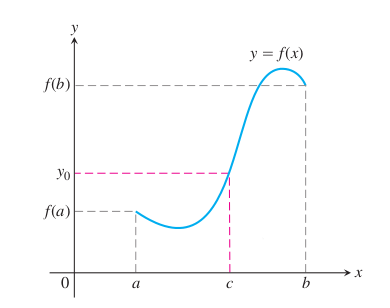
\includegraphics[height=4cm]{calc_multi_app_05.png}

Sezgisel olarak bu anlamlı değil mi? Eğer sürekli bir fonksiyon var ise,
$f(a)$'dan $f(b)$'ye giderken o aralıktaki her sayıya bir kez ``uğramaya''
mecburuz. Etraflarından dolaşmamız mümkün değil, çünkü kesintili bir
fonksiyon değil, kesintisiz / sürekli bir fonksiyonumuz var. Bu teorinin
daha detaylı ispatı için [1]'e bakılabilir. 

Maks-Min Eşitsizliği

Eğer $[a,b]$ aralığında $f$, maksimum değer $\max f$'e ve minimum değer
$min \ f$'e sahipse, 

$$ \min f \cdot (b-a) \le \int_a^b f(x) \ud x \le \max f \cdot (b-a) $$

demektir. 

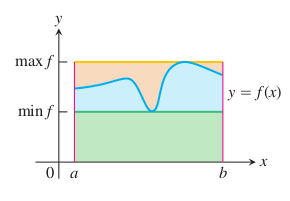
\includegraphics[height=4cm]{calc_multi_app_08.png}

Bu kural diyor ki $f$'in $[a,b]$ üzerindeki entegrali hiçbir zaman $f$'in
minimum'u çarpı $[a,b]$ aralığının uzunluğu'ndan küçük olamaz, ve $f$'in
maksimumu çarpı $[a,b]$ aralığının uzunluğu'ndan büyük olamaz. 

İspat

Eğer $(b-a)$'yi $ \sum_{k=1}^n \Delta x_k$ olarak görürsek

$$ \min \ f \cdot (b-a) = \min \ f \cdot \sum_{k=1}^n \Delta x_k $$
$$  = \sum_{k=1}^n \min \ f \cdot \Delta x_k  $$

$[a,b]$ aralığındaki herhangi bir değer $c_k$ için

$$  \le \sum_{k=1}^n f(c_k) \cdot \Delta x_k  $$

Öyle değil mi? $min \ f$ değeri en küçük değer ise, $[a,b]$ aralığındaki
herhangi bir nokta $c_k$'nin $f$ değeri bu değere ya eşit, ya da ondan
büyüktür. Yani $min \ f \le f(c_k)$. Devam edersek

$$  \le \sum_{k=1}^n \max f \cdot \Delta x_k  $$

Üstteki benzer mantığı takip ediyor, bu sefer $f(c_k) \le \max f $. Son
ifadedeki $max$'i dışarı alabiliriz. 

$$ = \max f \sum_{k=1}^n \cdot \Delta x_k  $$

$$ = \max f (b-a)  $$

Rolle'nin Teorisi

Bir sonraki teoriyi ispatlamadan önce orada gerekli Rolle'nin Teorisinden
bahsetmek lazım. Bu teoriyi ispatlamadan vereceğiz, kabaca doğru olduğunu
anlayabiliriz, teori der ki, eğer bir fonksiyon $f$ 1) $[a,b]$ kapalı bölgesinde
sürekli 2) (a,b) açık aralığında türevi alınabilir ve $f(a)=f(b)$ ise o zaman
bir aynı aralıkta $f'(c)=0$ olacak şekilde bir $c$ varlığı kesindir.

Altta bazı örnekler görüyoruz,

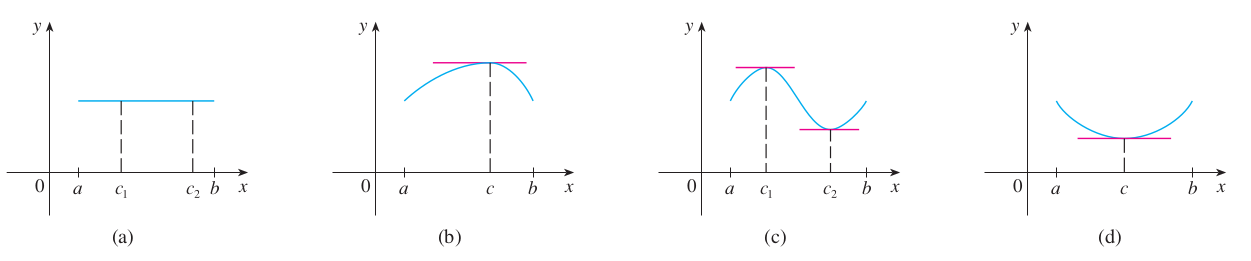
\includegraphics[width=30em]{calc_multi_app_02.png}

Tarif etmek gerekirse iki nokta arasında başı ve sonu aynı olan bir fonksiyon o
arada bir noktada muhakkak tepe, ya da dip noktasına varmış olmalıdır, yani
türevi orada sıfır olmalıdır. Bu sezgisel olarak akla yatkın bir önerme
herhalde. İspat için [2, sf. 281].

Ortalama Değer Teoremi (Türevli Form)

Eğer $f$ fonksiyonu açık aralığında (interval) $(a,b)$ türevi alınabilir halde
ise ve kapalı aralıkta $[a,b]$ sürekli ise, o zaman $(a,b)$ aralığında
en az bir $c$ değeri vardır ki bu değer için

$$
f'(c) = \frac{f(b) - f(a)}{b-a}
$$

doğrudur.

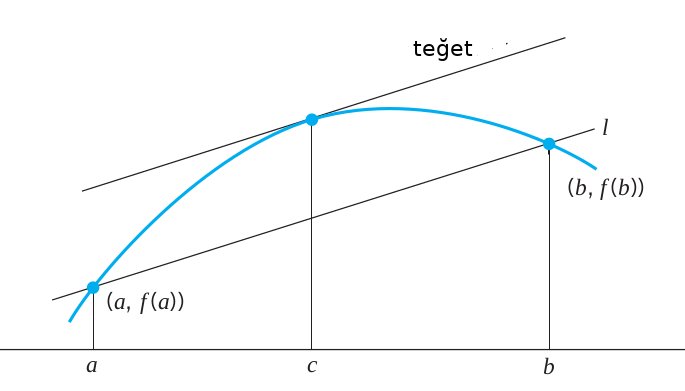
\includegraphics[width=20em]{calc_multi_app_01.png}

Bu teorinin de ispatı için [2, sf. 282]'ye bakılabilir, fakat yine kabaca takip
edilen tekniği tarif edeilm; eğer üstteki grafiği sağa doğru yatırırsak, yani o
$l$ çizgisi tam $x$ eksenine paralel olacak şekilde saat yönüne doğru her şeyi
çevirirsek, yeni $f(a)$ ve $f(b)$ aynı $y$ seviyesinde olacaklar, eh bu durumda
Rolle Teorisi kullanılabilir, ve oradan gelen $c$ olma mecburiyetini ilk
grafiğe tercüme edersek oradaki $c$ varlığını da ispatlamış oluruz. 

Ortalama Değer Teoremi (Entegral Form)

Eğer $f$ fonksiyonu $[a,b]$ arasında sürekli ise o zaman $[a,b]$ aralığında
olan bir $c$ noktasında

$$ f(c) = \frac{1}{b-a}\int_a^b f(x) \ud x $$

eşitliği doğru olmalıdır. Yani alttaki resimde sol grafikteki mavi alanın
$b-a$ ile bölünerek elde edilen ortalama değeri, $[a,b]$ aralığındaki bir
$c$ üzerinden $f(c)$'ye muhakkak eşittir. Ya da bir kenarı $f(c)$, diğeri
$b-a$ olan bir diktortgenin alanı (alt sağdaki resim), mavi alanın
tamamına eşit olacaktır.

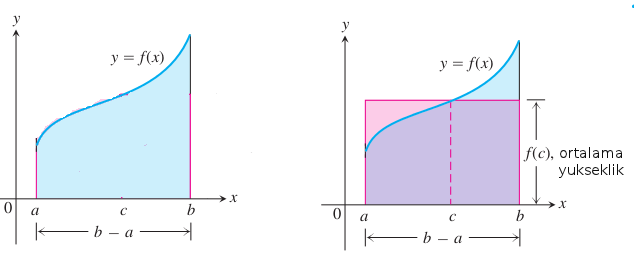
\includegraphics[height=4cm]{calc_multi_app_07.png}

Maks-Min Eşitsizliğinin iki tarafını $b-a$'ya bölersek

$$ \min f  \le \frac{1}{b-a} \int_a^b f(x) \ud x \le \max f  $$

elde ederiz. Eğer Geçiş Değeri Teorisi doğruysa, $\min f$ ve $\max f$
arasındaki tüm noktalar ziyaret edilmelidir. O zaman böyle bir $f(c)$
kesinlikle var demektir.

Calculus'un Temel Teoremi

Teori

Eğer $f$ fonksiyonu $[a,b]$ arasında sürekli ise o zaman 

$$ F(x) = \int_a^x f(t) \ud t  $$

fonksiyonu da $[a,b]$ arasında süreklidir, ve bu fonksiyonun türevi
$f(x)$'in kendisidir.

Yani

$$ F'(x) = \frac{d}{dx}\int_a^x f(t) \ud t = f(x)   $$

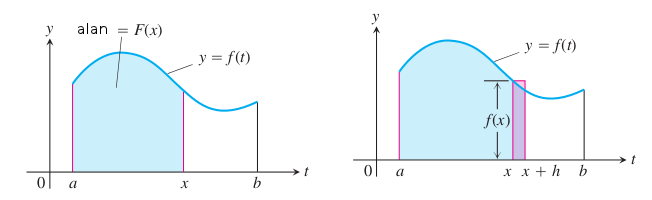
\includegraphics[height=3cm]{calc_multi_app_03.png}

İspat

Türevin tanımını direk $F(x)$ üzerinde uygulayalım, $[a,b]$ içinde olan $x$
ve $x+h$ aralığını alalım, ve

$$ \frac{F(x+h)-F(x)}{h} $$

bölümünün limitinin, $h \to 0$ iken, $f(x)$'e gittiğini göstermeye
çalışalım. $F(x+h)$ ve $F(x)$ fonksiyonlarını entegralleri üzerinden
tanımlayalım. O zaman üstteki formülün bölüm kısmı

$$ F(x+h) - F(x) = \int_a^{x+h} f(t) \ud t - \int_a^x f(t) \ud t  $$

Entegrallerin toplam kuralına göre üstteki formülün sağ tarafı 

$$ \int_x^{x+h} f(t) \ud t  $$

ifadesidir. O zaman bölümün tamamı

$$ \frac{F(x+h)-F(x)}{h} = \frac{1}{h} \int_x^{x+h} f(t) \ud t   $$

Ortalama Değer Teoremine göre, üstteki eşitliğin sağındaki ifadenin, $x$ ve
$x+h$ aralığında $f$'in aldığı değerlerden birine aynen eşit olduğunu
biliyoruz. Yani o aralıktaki bir $c$ için

$$ \frac{1}{h} \int_x^{x+h} f(t) \ud t = f(c) $$

kesinlikle doğru olmalı. Şimdi, $h \to 0$ oldukça, $x+h$ mecburen $x$'e
yaklaşmak zorunda kalacaktır, çünkü $c$, $x$ ile $x+h$ arasında sıkışıp
kalmıştır. $f$ fonksiyonu $x$ noktasında sürekli olduğuna göre, o zaman
$f(c)$, $f(x)$'e yaklaşmalıdır. 

$$ \lim_{h \to 0} f(c) = f(x) $$

Şimdi elimizdeki bu bilgiyle başa dönersek, 

$$ \frac{dF}{dx} = \lim_{h \to 0} \frac{F(x+h)-F(x)}{h} $$

$$  = \lim_{h \to 0} \frac{1}{h} \int_x^{x+h} f(t) \ud t   $$

$$ = \lim_{h \to 0} f(c) $$

$$ = f(x) $$

Ek olarak ilgili bir teori daha gösterelim.

Cauchy Ortalama Değer Teorisi (Cauchy Mean-value Theorem)

Teori şöyle

Eğer $f,g$ fonksiyonları $[a,b]$ aralığında sürekli ise ve $g'(x) \ne 0$
farz edildiği durumda $[a,b]$ arasında öyle bir $c$ vardır ki,

$$ \frac{f'(c)}{g'(c)} = \frac{f(b)-f(a)}{g(b)-g(a)} $$

ifadesi doğrudur. 

İspat

Şimdi daha önceden gördüğümüz Ortalama Değer Teorisi'ni (Cauchy olmayan)
iki kere kullanacağız. Teoriyi önce $g(a) \ne g(b)$ olduğunu göstermek için
kullanacağız. Çünkü eğer bu doğru olsaydı, Ortalama Değer Teorisi 

$$ g'(c) = \frac{g(b) - g(a)}{b-a} = 0$$

olurdu, ki bu $[a,b]$ arasındaki bir $c$ için başta yaptığımız faraziyemiz
$g'(x) \ne 0$ ile ters düşerdi. 

İkinci kullanım: $F(x)$ adında, $f,g$ fonksiyonlarını kullanan başka bir
fonksiyon kurgulayalım.

$$ F(x) = f(x) - f(a) - \frac{f(b)-f(a) }{g(b)-g(a)}[g(x)-g(a)] $$

Bu fonksiyonun türevi, $f,g$'nin türevi alınabildiği her yerde alınabilir
olur. Ayrıca $F(b) = F(a) = 0$. $a,b$ değerlerini yerine koyarsak bunu
görebiliriz, mesela $x=a$ için

$$ F(a) = \cancelto{0}{f(a) - f(a)} -
\frac{f(b)-f(a) }{g(b)-g(a)}
[\cancelto{0}{g(a)-g(a)}] 
$$

$$  = 0 - 0 = 0 $$

O zaman, $F(b) = F(a) = 0$'dan bir sonuca daha erişiriz. Bir fonksiyon
$a,b$ uçlarında sıfır ise, bu fonksiyon bir şekilde azalıp, çoğalıyor, ya
da çoğalıp azalıyor demektir, yani kesinlikle bir yerde tepe yapıyor
demektir. Tepe yapmanın Calculus'taki tercümesi $[a,b]$ arasındaki bir $c$
için $F'(c)=0$ olmasıdır. O zaman üstteki $F(x)$'in türevini alırsak, ve
$x=c$ dersek, 

$$ F'(c) = f'(c) - \frac{f(b)-f(a)}{g(b)-g(a)}[g'(c)] = 0$$

doğru olmalıdır. Türev alırken $f(a)$ yokoldu çünkü sabitti, büyük bölüm
yerinde kaldı çünkü tamamı $g(x)$ için katsayı. Eğer tekrar düzenlersek,
negatif terimi sola alırsak, ve iki tarafı $g'(c)$'ye bölersek,

$$ \frac{f'(c)}{g'(c)} = \frac{f(b)-f(a)}{g(b)-g(a)} $$

ifadesini elde ederiz. Yani baştaki teoriyi elde etmiş oluruz. 

Ortalama Değer Teorisini ilk kez kullanmamızın sebebi, üstteki bölenin sıfır
olmamasını istediğimiz içindi, çünkü sıfırla bölüm tanımsızdır. 

Türev İşlevi Nasıl Türetilir

Calculus, bir veya daha fazla dereceli denklemlerin, en yüksek noktasını
bulmak, değişimi temsil etmek gibi birçok bilim ve mühendislik alanında
kullanılır. Herhalde Calculus'in türev, entegral alma gibi yöntemlerini
şimdiye kadar çok gördük. Fakat genelde anlatılmayan, türev ve entegral
işlemlerinin nasıl yapıldığı, yani Calculus'in nasıl işlediği.

Örnek olarak, aşağıdaki grafiğe bakalım. 

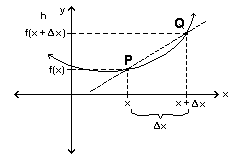
\includegraphics[height=4cm]{ode_mattuck_93_diff_10.png}

Gösterilen eğri, $x^2$ eğrisi. Bu eğrinin artış oranını bulmak için, artış
oranını temsil eden işlevi bulabiliriz. Bu işleve türev alarak gideceğiz.

Bunu yapmanın bir yolu, y eksenindeki artışı x eksenindeki artış ile
bölmek. 

$$ f(x) = x^2 $$

$f(x)$'in türevini bulmak için 

$$ = \frac{f(x+\Delta x) - f(x)}{\Delta x} $$

$$ = \frac{(x+\Delta x)^2 - x^2}{\Delta x} $$

$$ = \frac{x^2 + 2x\Delta x + \Delta x^2 - x^2}{\Delta x} $$

$x^2$'ler iptal oldu

$$=  \frac{2x\Delta x + \Delta x^2}{\Delta x} $$


$$ = 2x + \Delta x $$

Bu elimizdeki işlev, türevin son haline yaklaştı. En son haline getirmek
için, şöyle düşünmemiz gerekiyor. Artış miktarını bulduk, ama x eksenindeki
artış basamağı ne kadar büyük olmalı? Sonuna kadar küçültürsek, elimize
hangi işlev geçer?

Calculus'u ilk bulan Leibniz adlı matematikçi, zamanına göre büyük bir
ilerleme olan bu yeni metodu bir türlü meslektaşlarına tarif
edemiyordu. "$x^2$'nin türevi nasıl 2x oluyor" gibi sorulara, artış miktarı
kavramını anlatıyor, fakat $2x$ formülüne geldiğini bahsederken, "$x$'teki
artış sonsuz küçüldüğü için $2x$'e yaklaşıyoruz" deyince, arkadaşları onu
anlamıyordu. Zamanın matematikçileri bu 'sonsuz küçüklük' kavramını çok
eleştirdiler. Leibniz sonunda, "sonsuz küçük sayıların olduğu delilik gibi
gelebilir, fakat pratik hesaplamalar açısından yararlı bir alet olarak
Calculus'un hala yararlı olabileceğini düşünüyorum" demişti. Yani
Calculus'un matematiksel ispatı Leibniz zamanında yapılamadı. Keşifler
tarihin de bu olağan bir durumdur. Türevler, zamanı için yeterince normal
dışı bir buluştu, bunun üzerine hemen arkasından bir diğer sarsıcı buluşun
yapılması, çoğu zaman mümkün olmamaktadır.

Bu yüzden türevlerin soyut matematiksel olarak ispatının yapılması, 1821'de
limit kuramının keşfine kadar beklemiştir. Fakat bu keşiften önce bile,
mühendisler ve bilim adamları Calculus yöntemlerini verimli bir şekilde
kullanmaya başlamışlardı.

Sonsuz Küçüklük

Leipniz ve Calculus'un ``öteki babası'' sayılan Newton'un söylemeye
çalıştıkları, türev işleminin bir durağan resim üzerinde yapılan hesap
değil, ardışıl yaklaşıklama süreci altında bir sabit sonuca "yaklaşan"
hareketli bir hedef olduğu idi. Matematiksel limit kuramı, bu tür bir
tarifi gösterebildiği için sonunda Calculus'u ispatlamak mümkün oldu.

$$ g(x) = 2x + \Delta x $$

$$ \lim_{\Delta x \to 0}g(x) = \lim_{\Delta x \to 0} (2x + \Delta x)  $$

$$ \lim_{\Delta x \to 0}g(x) = 2x$$

Bu formüle bakarak bir daha belirtmek gerekir ki, $x$ değişimini 0'a
eşitlemiyoruz. 0'a eşitleseydik, daha baştan bölünen olarak elimize sıfır
geçeceği için cebirsel işlemde bu kadar ilerlememiz mümkün
olmazdı. Yaptığımız, limit tarifini kullanarak, $x$ sıfıra yaklaşırken
türev $2x$'e yaklaşır demektir.

Bu tanım sonucu elde ettiğimiz yeni fonksiyon da, tüm diğer fonksiyonlar
gibi, aynen limitlerin çalıştığı uzayda olduğu gibi sonsuz küçük
aralıklarla çalışabilecek bir tanım olduğu için, bu türetilmiş yeni
fonksiyonu da normal bir fonksiyon olarak kabul etmemiz mümkün olmaktadır.


Dolaylı Türev Almak (Implicit Differentiation)

Türev alırken başlangıçta $y = x^2$ turu $y$'yi direk $x$ ile ilintilendiren
açık, belirtilmiş, belli (explicit) fonksiyon varlığı farz edilir. Fakat bazen
elde dolaylı $x^2+y^2 = 9$ gibi bir fonksiyon olabilir burada her iki değişken
arasında bir alaka vardır fakat bağımlı, bağımsız değişken yoktur, gösterilen
ilişkiyi tatmin eden tüm $x,y$ değerleri geçerli değerlerdir. 

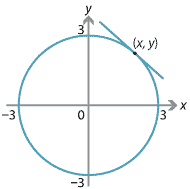
\includegraphics[width=20em]{ode_mattuck_93_diff_03.png}

Fakat bu durumda herhangi bir $x,y$ noktasındaki eğriye teğet çizgiyi nasıl
buluruz? Dolaylı türev alarak bunu başarabiliriz [4], yine $\frac{\ud}{\ud x}$
türevini alıyoruz ve uzun uzadıya $y$'yi $x$ üzerinden bir sürü cebirsel takla
ile temsil etmeye uğraşmadan türev işlemi bu alakayı farz ediyor, ve gerektiği
yerde Zincirleme Kuralı kullanıyor.

$$
\frac{\ud}{\ud x} (x^2)  + \frac{\ud}{\ud x} (y^2) = \frac{\ud}{\ud x} (9)
$$

İlk terim basit, $2x$. İkinci terimde Zincirleme Kuralı lazım,

$$
\frac{\ud}{\ud x} (y^2) = \frac{\ud}{\ud x} (y^2) \frac{\ud y}{\ud x} =
2y \frac{\ud y}{\ud x}
$$

Üçüncü terim sabitin türevi olduğu için sıfır. Yani

$$
2x + 2y \frac{\ud y}{\ud x} = 0
$$

Şimdi $\ud y / \ud x$ için düzenleme yaparsak,

$$
\frac{\ud y}{\ud x} = -\frac{x}{y}
$$

elde ederiz.

Entegralleri Türetmek

Aynen türevleri limitler üzerinden formalize edebildiğimiz gibi
entegralleri de toplamların eriştiği bir limit olarak formalize
edebiliriz. Bu bakış açısını matematiksel olarak tarif eden Bernhard
Riemann'dir ve tarif ettiği entegral formalizmi Riemann toplamı (Riemann
sum) olarak bilinir [1, sf. 340]. 

Diyelim ki bir $f(x)$ fonksiyonumuz var, iki nokta arasındaki $x$ yatay
eksenini $\Delta x$ büyüklüğünde $n$ tane eşit parçaya bölüyoruz, her parça
ortasındaki $c_k$'de fonksiyonun değeri tabii ki $f(c_k)$, bu dikdörtgen
parçasının yüksekliği, genişliği $\Delta x$. Riemann formalizmi için bu
parçaların eşit büyüklükte olması gerekmez, biz alttaki örnek için eşit
diyeceğiz, ve

$$ 
I = \lim_{n \to \infty} \sum_{k=1}^{n} f(c_k) \Delta x
$$

hesabına bakacağız.

Entegralleri Nasıl Düşünelim

Calculus kitaplarında entegralleri anlatmak için çoğu zaman ``toplam''
kavramı on plana çıkarılır, mesela entegralin alttaki resimde $f(x)$
fonksiyonunun altında kalan ufak ufak dikdörtgenlerinin alanlarının
``toplamı'' olduğundan bahsedilir.

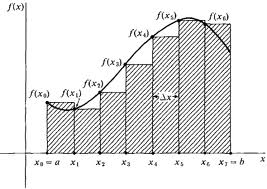
\includegraphics[height=4cm]{area.png}

Fakat bu tür bir anlatım bazen karışıklığa yol açabiliyor [6]. Daha iyi bir
anlatım entegralin ``değişen değerlerin çarpımı'' olduğudur. Alttaki
resimdeki dikdörtgeni düşünelim, 

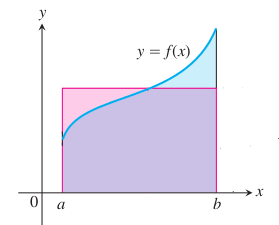
\includegraphics[height=4cm]{box.png}

ve diyelim ki bir dikdörtgen, entegralin hesapladığı alanı yaklaşıksal
olarak temsil ediyor. Dikdörtgen alanı nasıl hesaplanır? İki kenarının
çarpılmasıyla! Entegral de aslında böyle bir hesaptır, sadece kenarlardan
biri sabit değildir, ve sürekli değişmektedir. Bu tür bir anlayış birimleri
sonuca dahil etmek gerektiğinde ise yarar, mesela yatay ekşen zaman $t$
işe, ve dikey eksen hız $v(t)$ ise, katedilen mesafe, $v(t)$ nasıl bir
şekilde verilmiş olursa olsun,

$$ Mesafe = \int v(t) \ud t $$

formülüyle hesaplanacaktır. Eğer hız ve zaman sabit olsalar, mesela 5 ile 4
gibi, o zaman hesap son derece basit olacaktı, 3 x 4 = 12 ile sonucu
bulacaktık. 

Tabii ki çarpmak ile toplamak arasında yakın bağlantılar var, mesela 3 x
4'u şu şekilde resmedelim

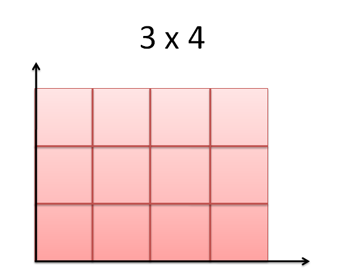
\includegraphics[height=4cm]{ode_mattuck_94_int_04.png}

Burada, evet, 3 değerini dört kere birbiriyle topluyoruz, 3 + 3 + 3 + 3 =
12 ve bu durum 3 x 4 ile aynı sonucu veriyor. Fakat 3'lerin toplamı, eğri
altındaki alan zihniyetini daha ilerletmeden azıcık farklı bir durumu
düşünelim. 

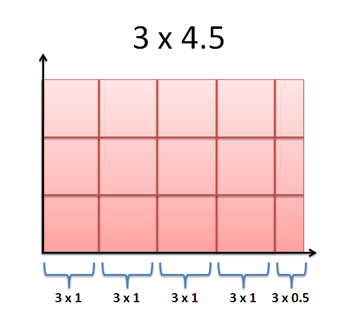
\includegraphics[height=4cm]{ode_mattuck_94_int_09.png}

Bu durumda dikey eksendeki kolonlara bir ek yaptık, ama bu ekin genişliği
tam bir kolon değil, yarım bir kolon. Bu durumda alan hesabını sadece dikey
kolonların toplanması olarak yapsakdik 3'u beş kere toplamamız gerekirdi,
ve 15 elde ederdik, yanlış bir hesap yapmış olurduk.

Toplamın doğru olması için yatay ekşenin genişliğinin hesaba katılması
gerekir, 3*1 + 3*1 + 3*1 + 3*1 + 3*0.5 = 13.5. Ya da tüm genişliği tüm
yükseklik ile çarparız 3 * 4.5 = 13.5. 

Peki ilk örneğe dönersek, madem çarpımlardan bahsediyoruz, diyelim ki
$v(t) = 2t$ o zaman $t \cdot 2t$ diyemez miyiz? Bu da olmaz, çünkü $t\cdot 2t = 2t^2$ 
bize sadece tek bir $t$ anındaki bir hesabı veriyor. Biz verilen bir 
başlangıç ve bitiş noktaları arasındaki ``tüm $t$'ler üzerindeki'' 
katedilen mesafeyle ilgileniyoruz.  

Yani entegral denince aklımıza çarpım gelsin, $x,y$ eksenleri bağlamında,
$y$ eksenindeki $f(x)$'i $x$'i çarpıyoruz, bu çarpım $x$ için entegrale
$dx$ olarak yansıyor, $f(x)$ ise entegre edilen fonksiyon haline geliyor. 

Birimleri hesaba katarsak anlatılanlar biraz daha anlamlanır belki. Eğer
hız km / saat ise, zaman saat ise, sadece hızların toplamı mesafe birimini
km / saat yapar, bu yanlış olur. Ama çarpım olarak düşünürsek km / saat *
saat = km sonucunu verir ki bu mesafenin birimidir. 

Ortalama mı, Toplam mı?

Diğer yandan bazen bir aralıkta bir fonksiyonun entegrali alındığında onun
``ortalamasından'' da bahsedildiğinin görebiliriz. Peki bir entegral bir
toplam midir (ya da akıllı çarpım) yoksa bir ortalama mı? Aslında bu iki
kavram arasında fazla bir fark yok; sonuçta 10 tane sayının toplamı ile
averajı arasında 1/10 sabiti ile çarpım haricinde bir fark yok [7]. 

Tam Diferansiyel (Total Differential)

Bir $f$ fonksiyonunun tam diferansiyeli (total differential) o
fonksiyonun lineerleştirilmesi anlamına gelir. İki değişkenli bir
fonksiyon için şöyle temsil edilir:

$$ df = f_x(x_0, y_0)\ud x + f_y(x_0,y_0)\ud y  $$

Bu formu nasıl türetiriz? Bize lazım olan lineerleştirme formülasyonu. Tek
değişkenli bir fonksiyonu lineerleştirmenin tekniği şudur:

$$ L(x) = f(x_0) + f'(x_0) \Delta x  $$

Burada $L(x)$ gerçek fonksiyonu yaklaşıksal (approximate) olarak temsil eden
lineer fonksiyondur. 

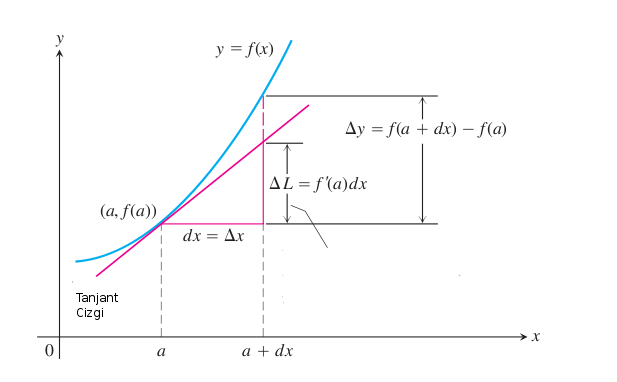
\includegraphics[height=6cm]{ode_mattuck_95_total_06.png}

Bu fonksiyonu genişleterek iki değişkenli hale getirelim (sadece $y$
ekleyeceğiz)

$$ L(x,y) = f(x_0,y) + f_x(x_0,y) \Delta x $$

Bu fonksiyon da bir önceki kadar ``geçerli''. Sonuçta fonksiyonlar
noktasal değerlere göre sonuç verirler, bu sebeple bir lineerleştirme
işlemi 2 boyutlu ortamda herhangi bir $x$ noktasında yapılabildiği
gibi, herhangi bir $x$, $y$ noktasında da yapılabilir.

Şimdi üstteki denklemin sağ tarafında yer alan $f(x_0,y)$'yi lineerleştirelim.  

$$ L(x,y) = L(x_0,y_0) + f_y(x_0,y_0) \Delta y + f_x(x_0,y_0) \Delta x $$

Artık $L(x_0,y_0)$'yi sol tarafa taşıyabiliriz:

$$ \Delta L = L(x,y) - L(x_0,y_0) = f_y(x_0,y_0) \Delta y + f_x(x_0,y_0)
\Delta x $$ 

$\Delta L$ yani $df$ istediğimiz tam diferensiyel sonucudur, $\Delta
x$ yerine $\ud x$, $\Delta y$ yerine $\ud y$ kullanabiliriz, o zaman baştaki
formun aynısını elde etmiş oluruz.

Türetirken kullandığımız numarayı üç, dört, vs. gibi istediğimiz kadar
değişken taşıyan $f$ fonksiyonları için yapabilirdik, ve sonuç üstteki
forma benzer olurdu. Her değişkenin kısmi türevi o değişkenin sonsuz
ufaklıktaki ``değişimi'' ile çarpılıp, o çarpımlar toplanınca elimize
tam diferansiyel geçiyor.

Bu yazı [1, sf. 130], [1, sf. 347], [1, sf. 358], ve [1, sf. 257]'yi baz
almıştır. Diğer kaynaklar altta. 

$dy/dx$ bir kesir olarak görülebilir mi? 

Mesela [1, sf. 225] bölüm 3.8'te türev $dy/dx$'in bir kesir, bir oran
olmadığı söylenir. Fakat bu şekilde görülemez mi? Çünkü $dy = f'(x)dx$
formülünde $dx$ için gerçek sayılar verip sonucu (diferansiyeli) $dy$
olarak hesaplayabiliyoruz. Eğer bu formülü tekrar düzenlersek $dy/dx$ for
kesir olarak görülebilirdi.. belki.

Fakat bu teorik olarak tamamiyle, her zaman işlemiyor. Yani pratikte bazen
bu şekilde görebiliyoruz, fakat işin en temelinde durum böyle değil.

Tarihsel olarak, Calculus'u keşfeden matematikçi Leibniz bu notasyonu ileri
sürdüğünde $dy/dx$'i bir kesir olarak düşünmüştü, bu değerin temsil ettiği
büyüklük ``$x$'deki sonsuz ufak (infinitesimal) değişimin $y$'de yarattığı
sonsuz ufak değişime oranı'' olarak düşünülüyordu.

Fakat Calculus'un sonsuz ufaklıklar mantığını reel sayılar çerçevesinde
kullanmak teorik olarak pek çok problemi beraberinde getiriyor. Bunlardan
biri, sonsuz ufaklığın reel sayıların olduğu bir çerçevede var
olamamasıdır! Reel sayılar önemli bir önşartı yerine getirirler, bu şartın
ismi Arşimet Şartı'dır. Bu şarta göre, ne kadar küçük olursa olsun herhangi
bir pozitif tam sayı $\epsilon > 0$, ne kadar büyük olursa olsun reel bir
sayı $M>0$ bağlamında, $n\epsilon > M$ şartını doğrulayacak bir doğal sayı
$n$ her zaman mevcuttur. Fakat sonsuz ufak bir $\xi$ o kadar ufak olmalıdır
ki onu kendisine ne kadar eklersek ekleyelim, hiçbir zaman 1'e erişemeyiz,
ki bu durum Arşimet Şartına aykırı olur [..]

Bu problemlerden kurtulmak için takip eden 200 sene içinde Calculus ta
temelinden başlayarak sıfırdan tekrar yazılmıştır, ve şimdi gördüklerimiz
bu sıfırdan inşanın sonuçları (mesela limit kavramı bunun bir sonucu). Bu
tekrar yazım sayesinde / yüzünden türevler artık bir oran değil, bir limit.

$$ \lim_{h \to 0} \frac{f(x+h) - f(x)}{h}$$

Bu ``oranın limiti''ni ``limitlerin oranı'' olarak yazamayacağımız için
(çünkü hem bölüm, hem bölen sıfıra gidiyorlar), o zaman türev bir oran
değildir.

Fakat Leibniz'in notasyonu o tür kullanımı özendiriyor sanki, oraya doğru bir
çekim yaratıyor, hatta bazen notasyonu o şekilde görmenin işe yaradığı bile
oluyor, yani çoğu zaman bu notasyon sanki kesirmiş {\em gibi}
davranıyor. Zincirleme Kanunu mesela

$$ \frac{dy}{dx} = \frac{dy}{du}\frac{du}{dx} $$

Türevlerin kesir olarak görüldüğü bir durumda üstteki ifade hakikaten doğal
duruyor. Ya da Tersi Fonksiyon (Inverse Function) teorisi

$$ \frac{dx}{dy} = \frac{1}{\frac{dy}{dx}} $$

sonucu da eğer türevleri kesir olarak düşünüldüğü bir ortamda doğal
gelecektir. İşte bu sebeple, yani notasyonun çok güzel ve özendirdiğinin
çoğunlukla doğru şeyler olması sebebiyle artık bir limiti temsil eden
notasyonu kullanmaya devam ediyoruz, her ne kadar artık gerçekten bir
kesiri temsil etmiyor olsa bile. Hatta şu ilginç tarihi anektodu ekleyelim,
bu notasyon o kadar iyidir, Newton'un notasyonu olan tek tırnak ($y'$ gibi)
işaretinden o kadar ileridir ki bazılarının iddiasına göre İngiltere'deki
matematik ve bilim kara Avrupa'sının yüzyıllarca gerisinde kalmıştır -
çünkü Newton ve Leibniz arasında Calculus'u kimin keşfettiği konusunda bir
çatışma yaşandı (bugünkü konsensüs ikisinin de Calculus'u aynı anda
keşfettiği üzerine), ve bu çatışma ortamında İngiliz bilim çevresinin
Avrupa'daki ilerlemeleri, Leibniz notasyonunu dışlayıp Newton'u takip
etmeleri sonucunu getirdi.. ve bu sebeple pek çok alanda geri kaldılar
[..].

Sonuca gelirsek, $dy/dx$'i bir kesir gibi yazıyor, ve pek çok hesapta onu
sanki bir kesirmiş gibi kullanıyor, kullanabiliyor olsak bile, $dy/dx$ bir
kesir değildir, sadece filmerde o rolü oynar (!).

Sonsuz Kuvvet, Calculus'un Temeli

Calculus'un bu kadar başarılı olmasının sebebi nedir? Calculus'un
başarısının altında yatan sır çetrefil problemleri ufak parçalara
bölebilmesi [8]. Tabii ki bir problemi parçalara bölmeyi pek çok diğer
alanda da görüyoruz. Ama Calculus bunu en radikal şekilde yapıyor,
problemleri {\em sonsuz ufak parçalara} bölebiliyor. Bir problemi bir, iki,
vs. parçaya bölmek yerine onu bölüyor, bölüyor, ta ki problem unufak sonsuz
tane parçalar haline gelinceye dek, sonra problemi o ufacık parçalar için
çözüyor, ki bu noktada çoğunlukla çözüm büyük problemden çok daha rahattır.
Sonra herşeyi biraraya koyuyor, bu adım bölmekten daha zor olabilir ama
yine de esas büyük problemi çözmekten daha kolaydır, ve çözüme ulaşılıyor.

Yani Calculus iki adımda işini yapıyor, bölmek ve biraraya koymak. Bölme
kısmına diferansiyel Calculus deniyor, biraya koyma kısmına entegral
Calculus.

Calculus aslında çok eskidir, çünkü biraz önce bahsettiğimiz prensibin
takip edilmesi için muhakkak formülsel formlar takip etmek şart
değil. Mesela M.Ö. 250 zamanında yaşamış Arşimet bir çemberin alanını aşağı
yukarı şöyle bir yaklaşımla buldu. Elimizde bir daire var, bir pizza
diyelim, bu pizzanın alanını bulmak istiyoruz,

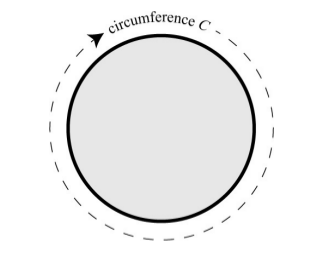
\includegraphics[height=4cm]{circ_1.png}

Bildiklerimiz pizzanın yarıçapı (radıus) $r$ ve çevresi $C$. Eğer pizzadan
ufak bir parça kessek parçanın iki yanı tabii ki $r$ olur.

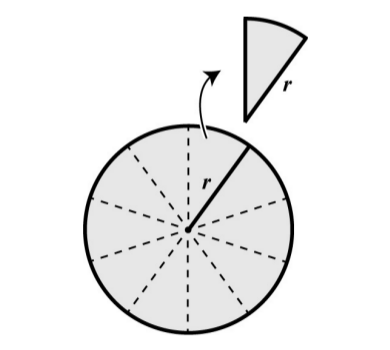
\includegraphics[height=5cm]{circ_2.png}

Alan hesabı yapmak istiyoruz, bir fikir şu, pizzayı dört parçaya bölelim,
sonra parçaları yanyana koyalım.

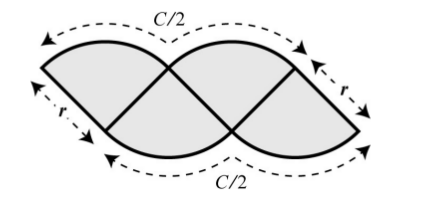
\includegraphics[height=3cm]{circ_3.png}

Bu pek düzgün bir şekil olmadı, alanı rahatça hesaplamak kolay değil. Emin
olduğumuz bir şey var, engebeli olsa da üst kısım $C/2$ uzunluğunda, alt
kısım aynı şekilde. Bir dikdörtgen olsa iyi olurdu, o şekle erişmemiş
olmamızın sebebi yeterince ufak parçaya bölmemiş olmamız mı acaba? 8
parçaya bölelim, ve yine parçaları yanyana koyalım,

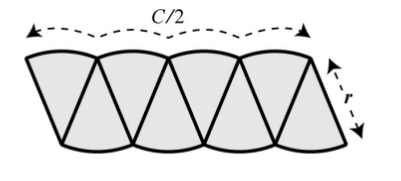
\includegraphics[height=3cm]{circ_4.png}

Bu şekil bir paralelogramı andırmaya başladı. Fena değil, üst, alttaki
sınırların engebesi azaldı, düzleşmeye başladılar. Aslında bir
dikdörtgenimsi sekle ufak bir hamle ile daha yaklaşabiliriz, soldaki
parçanın yarısını alıp sağ tarafa yapıştıralım,

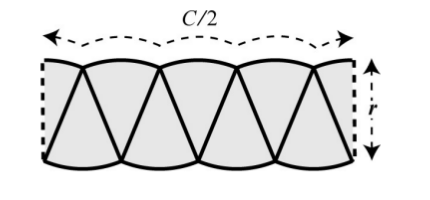
\includegraphics[height=3cm]{circ_5.png}

Güzel. Hala tam düzleşme elde edemedik, eh ama şimdiye kadar ufalta ufalta
bayağı yol aldık, daha da ufaltalım, 16 parça,

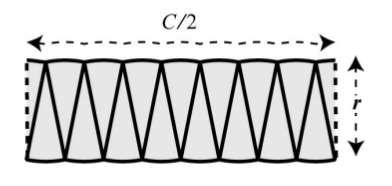
\includegraphics[height=3cm]{circ_6.png}

Ne kadar parçaya bölersek o kadar dikdörtgene yaklaşıyoruz. Üstteki şekil
dikdörtgene yaklaştığı için sonsuz parçanın birleşmesinin limite giderken
tam bir dikdörtgen olacağını biliyoruz. 

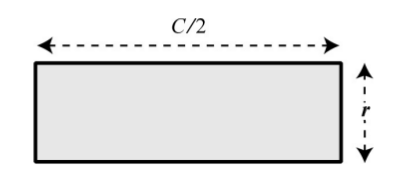
\includegraphics[height=3cm]{circ_7.png}

Bu dikdörtgenin alanını bulmak çok kolay, $r \cdot C/2$. Eh bölünen parçaları
kaybetmedik, hepsini kullandık, o zaman bu alan en baştaki dairenin de alanı
olmalı! Arşimet işte daire alanını, matematiksel ispatı ile beraber, işte böyle
hesapladı

Not: Formülleri daha detaylandırırsak, $C$'nin $r$ ile ilişkisi zaten
biliniyorsa, $C = 2 \pi r$, buradan alan

$$
A = r C/2 = r (2 \pi r)/2 = \pi r^2 
$$

Fakat $C$ bazlı alan ispatının en dahiyane kısmı sonsuzluğun kullanılma
şekli. 4, 8, 16 ile başladık, parçaların toplamı gitgide daha çok dikdörtgene
benzemeye başladı. Ama sonsuz tane parçanın limitinin ortaya çıkarttığı şekil
tam dikdörtgen olacaktı, ve nihai hesapta bu formu kullanabilirdik. İşte
Calculus'un temeli burada yatıyor. Sonsuzluğa gidince herşey daha basit hale
geliyor.



Kaynaklar

[1] Thomas, {\em Thomas Calculus 11th Edition}

[2] Stewart, {\em Calculus, Early Transcendentals}

[3] Strang, {\em Calculus}

[4] AMSI, {\em Implicit differentiation},
    \url{https://www.math.ucdavis.edu/~kouba/CalcOneDIRECTORY/implicitdiffdirectory/ImplicitDiff.html}

[6] Better Explained, {\em A Calculus Analogy: Integrals as  Multiplication},
    \url{http://betterexplained.com/articles/a-calculus-analogy-integrals-as-multiplication/}

[7] Quora, \url{https://www.quora.com/Is-an-integral-more-analogous-to-a-sum-or-to-an-average}

[8] Strogatz, {\em Infinite Powers}

\end{document}


